

\excercise{Einschub: Objekte, Klassen, Klassendiagramm}

\begin{Infobox}[HowTo: Klassen und Objekte auseinander halten]
    In Java (und auch in anderen Programmiersprachen) gibt es \textbf{Klassen} und \textbf{Objekte}.
    Dabei gehört ein Objekt immer zu einer Klasse. Genauer gesagt ist ein Objekt \textbf{eine Instanz} einer Klasse.

    Die Klasse beschreibt dabei generell welche Eigenschaften und Operationen ein Objekt haben kann.
    Eigenschaften können zum Beispiel Daten (wie der Name oder die Farbe des Objekts) sein.
    Operationen wiederum sind Funktionen die das Objekt ausführen kann.
    Das Objekt, also eine konkrete Instanz der Klasse, hat dann zum Beispiel eine bestimmte Farbe (z.B. grün).
    Ein anderes Objekt der selben Klasse kann eine eigene Farbe (z.B. rot) haben.\\

    Man muss sich dabei oft entscheiden wie generisch oder genau man eine Klasse macht. Zum Beispiel kann man die Klasse Sportschuh und die Klasse High Heels haben oder man hat nur eine Klasse Schuh mit einer Eigenschaft, welche die Schuhart beschreibt.
\end{Infobox}

\begin{enumerate}
    \item Wir haben hier ein paar Klassen. Bitte erweitere sie um je 3 weitere Eigenschaften. Der Stuhl ist ein Beispiel:

    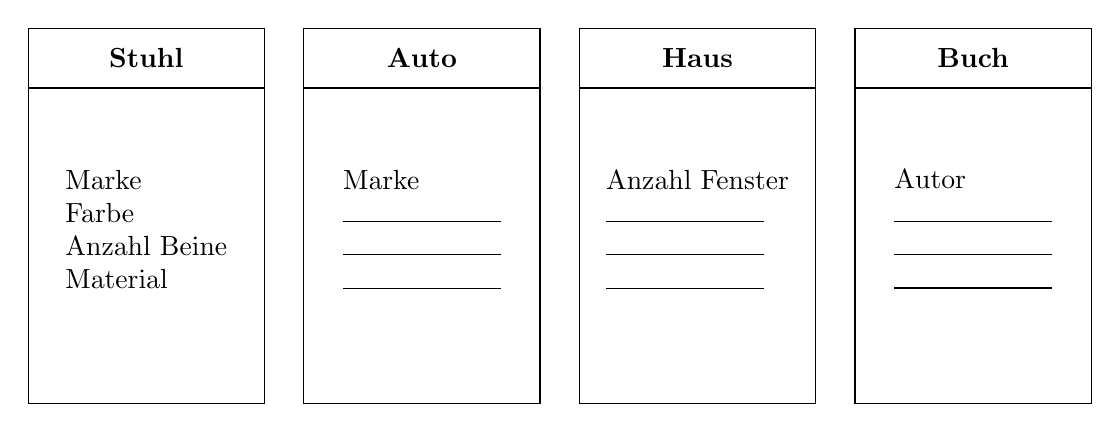
\begin{tikzpicture}
        \node[draw, rectangle, minimum height=0.75cm,minimum width=3cm, anchor=south] (A) {\textbf{Stuhl}};
        \node[draw, rectangle, minimum height= 4cm, minimum width=3cm,align=left, anchor=north] (B) {Marke\\Farbe\\Anzahl Beine\\Material\\};

        \node[draw, rectangle, minimum height=0.75cm,minimum width=3cm, anchor=south] (A1) at (3.5,0) {\textbf{Auto}};
        \node[draw, rectangle, minimum height= 4cm, minimum width=3cm,align=left, anchor=north] (B1) at (3.5,0) {Marke\\$\rule{2cm}{0.15mm}$\\$\rule{2cm}{0.15mm}$\\$\rule{2cm}{0.15mm}$\\};

        \node[draw, rectangle, minimum height=0.75cm,minimum width=3cm, anchor=south] (A1) at (7,0) {\textbf{Haus}};
        \node[draw, rectangle, minimum height= 4cm, minimum width=3cm,align=left, anchor=north] (B1) at (7,0) {Anzahl Fenster\\$\rule{2cm}{0.15mm}$\\$\rule{2cm}{0.15mm}$\\$\rule{2cm}{0.15mm}$\\};

        \node[draw, rectangle, minimum height=0.75cm,minimum width=3cm, anchor=south] (A1) at (10.5,0) {\textbf{Buch}};
        \node[draw, rectangle, minimum height= 4cm, minimum width=3cm,align=left, anchor=north] (B1) at (10.5,0) {Autor\\$\rule{2cm}{0.15mm}$\\$\rule{2cm}{0.15mm}$\\$\rule{2cm}{0.15mm}$\\};
    \end{tikzpicture}

    \item Nun erstelle zu jeder Klasse drei verschiedene Objekte. Wenn ihr in einer Gruppe zusammenarbeitet sollte sich jeder selbst ein Objekte ausdenken.

    \item Identifiziere im folgenden Text drei vorkommende Klassen mit jeweils drei Eigenschaften:

    Die BilligMöbel GmbH ist ein Unternehmen mit 1000 Mitarbeiter.
    In der Akte jedes Mitarbeiters ist sein Name und Alter sowie sein Gehalt und seine Kontonummer.
    Aufgrund von Massenproduktion  kann das Untenehmen ihre Möbel sehr Billig verkaufen.
    So kosten z.B. Stühle 10€, Liegen 15€ und Schränke 32€.
    Alle kann man aus Plastik oder Holz bekommen und in verschiedenen Farben.
    In ihrer Kundenkartei vermerken sie das Geschlecht und Postleitzahl ihrer Kunden sowie die Kosten ihres letzten Éinkaufs.
\end{enumerate}

\begin{Infobox}[HowTo: Operationen von Objekten]
    Klassen verfügen über Operationen die von bzw. auf ihren Objekten ausgeführt werden können.
    Als Beispiel betrachten wir ein Auto. Es kann fahren, bremsen, abbiegen oder den Motor an-/abschalten.\\

    Dabei können Operationen auch sogenannte Parameter besitzen wie z.B. abbiegen(links) oder fahren(50) (für 50 km/h).
    Wie man genau bestimmt was diese Parameter bedeuten erklären wir noch.
\end{Infobox}

\begin{enumerate} \setcounter{enumi}{3}
    \item Überlege dir für die folgenden 3 Klassen, Operationen.
    Es ist nicht notwendig Parameter zu verwenden.
    Der Stuhl ist wieder ein Beispiel:

    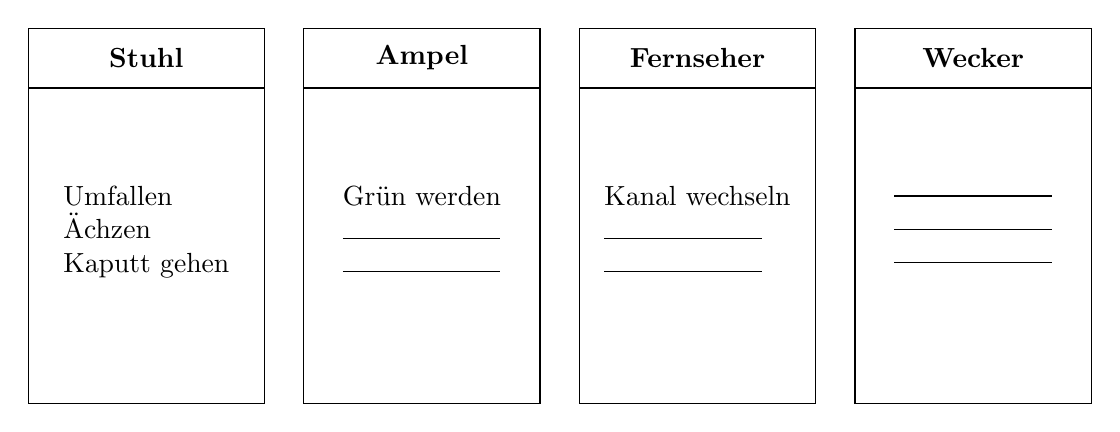
\begin{tikzpicture}
        \node[draw, rectangle, minimum height=0.75cm,minimum width=3cm, anchor=south] (A) {\textbf{Stuhl}};
        \node[draw, rectangle, minimum height= 4cm, minimum width=3cm,align=left, anchor=north] (B) {Umfallen\\Ächzen\\Kaputt gehen\\};

        \node[draw, rectangle, minimum height=0.75cm,minimum width=3cm, anchor=south] (A1) at (3.5,0) {\textbf{Ampel}};
        \node[draw, rectangle, minimum height= 4cm, minimum width=3cm,align=left, anchor=north] (B1) at (3.5,0) {Grün werden\\$\rule{2cm}{0.15mm}$\\$\rule{2cm}{0.15mm}$\\};

        \node[draw, rectangle, minimum height=0.75cm,minimum width=3cm, anchor=south] (A1) at (7,0) {\textbf{Fernseher}};
        \node[draw, rectangle, minimum height= 4cm, minimum width=3cm,align=left, anchor=north] (B1) at (7,0) {Kanal wechseln\\$\rule{2cm}{0.15mm}$\\$\rule{2cm}{0.15mm}$\\};

        \node[draw, rectangle, minimum height=0.75cm,minimum width=3cm, anchor=south] (A1) at (10.5,0) {\textbf{Wecker}};
        \node[draw, rectangle, minimum height= 4cm, minimum width=3cm,align=left, anchor=north] (B1) at (10.5,0) {$\rule{2cm}{0.15mm}$\\$\rule{2cm}{0.15mm}$\\$\rule{2cm}{0.15mm}$\\};
    \end{tikzpicture}

    \item Überlege dir nun eine eigene Klasse und finde zu ihr 3 Eigenschaften und 3 Operationen. Dann überlege die 3 Objekte dieser Klasse. Wenn du in einer Gruppe arbeitest könnt ihr gerne durchtauschen und jeder muss Objekte für die Klasse eines Kommilitonen finden.

    \begin{Infobox}[Info: Objekte vs. reale Objekte]
        Wichtig zu verstehen ist das Klassen und Objekte keine physischen Objekte repräsentieren müssen. Man kann auch z.B. eine Klasse für User Accounts oder eine Klasse für Personengruppen haben. Auch werden Klassen verwendet um technische Teile des Programms zu repräsentieren wie z.B. Das Fenster das angezeigt wird oder ein Paket das durchs Internet geschickt wird.
    \end{Infobox}

    \item (optional) Versuche erneut 3 Klassen mit je 3 Eigenschaften  zu identifizieren. Diese Aufgabe soll etwas schwieriger sein als die c)
    \paragraph{}
    Du betrittst die Gebäude und schaust dich um. Es gibt sehr viele Menschen hier. Doch niemanden den du kennst, also bewegst du dich direkt auf den Aufzug zu. Doch bevor du in dein Stockwerk fahren kannst musst du deine Personalkarte vor den Leser halten. Nachdem deine Sicherheitsstufe ausgelesen wurde kannst du den Knopf für das 5. Stockwerk drücken. Langsam fährt der Aufzug los. Langsamer als sonst. Larry wird ihn wohl wieder neu eingestellt haben.

    Im 5. Stockwerk angekommen erwartet dich ein Sicherheitsposten. Er ist nur mit einer statt mit 2 Personen besetzt, doch das macht dir keine Sorgen. Immerhin ist es Sonntag. Der Mann fragt nach deiner Personalkarte und scannt sie. Auf seinem Bildschirm taucht ein Foto auf, das er mit deinem Gesicht vergleicht. Doch ihm fällt nichts auf also grüßt er dich und lässt dich vorbei. Für einen Moment fragst du dich woher er deinen Namen kennt, doch der wurde vermutlich einfach mit dem Foto angezeigt. Heute ist einfach alles auf diesen Karten gespeichert.

    Du schlenderst durch das Labyrinth aus Gängen bis du zu deinem Ziel kommst. Die Tür ist unscheinbar und das Büro dahinter ist es auch. Kaum 10 Quadratmeter groß. Und die Fenster zeigen auf nichts beachtenswertes. Aber das ist dir Egal. Dich interessiert der Tresor in der obersten Schublade des Schreibtisch. Ein Model 4452 von SuperSecure.

    Du versicherst dich kurz das die Tür zu ist und dann machst du dich an das knacken des digitalen Schloss. Es dauert kaum 2 Minuten dann schwingt die 3cm dicke Stahltür auf und ermöglicht die Sicht auf ein duzend USB-Sticks. Schnell suchst du den blauen mit 16 GB Kapazität und lässt ihn in deiner Hosentasche verschwinden.

    Jetzt nur noch den gleichen Weg zurück.
\end{enumerate}
